\subsection{Adding a Class to Your Project}
First you have to create a package for your class files. Select the project you created in the section \ref{creating_project} in the package explorer. Right click on it and select \markedtext{New} $\rightarrow$ \markedtext{Other} from the context menu. You have to look for \markedtext{Package} in the \markedtext{Java} subsection as you can see in figure \ref{fig:package}.

\begin{figure}[htbp]
	\centering
		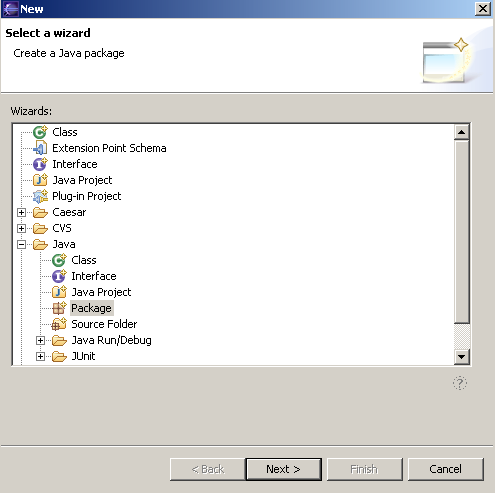
\includegraphics[width=0.60\textwidth]{images/package.png}
	\caption{Creating a package}
	\label{fig:package}
\end{figure}

Name the package \code{myPackage} then click \markedtext{Finish}.\\
Right-click on the package you have just created and select \markedtext{New} $\rightarrow$ \markedtext{Class} from the context menu. Name the class \code{HelloWorld} and activate the option to let Eclipse create a new main method for you. Click \markedtext{Finish}.
Edit the text in the editor so that it looks like this:
%\begin{table*}[htbp]
	\begin{lstlisting}[basicstyle=\small\it,caption=HelloWorld.java,label=lst:HelloWorld,name=listing:helloworld,frame=none]{}
package myPackage;

public cclass HelloWorld {
	private static HelloWorld instance = new HelloWorld();
	
	public void sayHelloTest(String message) {
		System.out.println(message);
	}
}
\end{lstlisting}
%	\caption{HelloWorld.java}
%	\label{lst:HelloWorldJava}
%\end{table*}
Save the file.\\
Notice that unlike in a Java project, there was no eager parsing of the buffer while you were typing. Also the outline view didn't update.\footnote{The \caesarj ~outline bar requires meta information from the compiler to display crosscutting relationships.} Your Eclipse workbench should be looking somehow like in figure \ref{fig:workspace_newclass}.\\

\begin{figure*}[htbp]
	\centering
		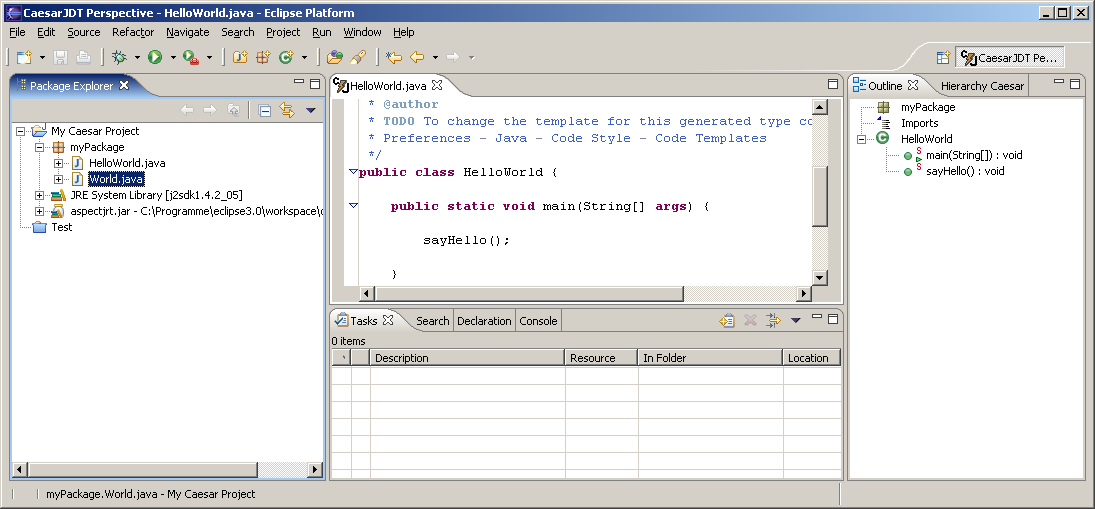
\includegraphics[width=1.0\textwidth]{images/workspace_newclass.png}
	\caption{Workbench with HelloWorld.java}
	\label{fig:workspace_newclass}
\end{figure*}
